\section{Методика решения}

\subsection{Подход}

В работе было предложено предсказывать амплитуды дифракционных максимумов, которые нельзя получить из эксперимента, по известным из того же эксперимента. После предсказания достаточного количества отражений, разрешения данных должно хватить для определения фаз и расчета электронной плотности одним из рутинных ab initio методов, в качестве которого был выбран метод, реализованный в комплексе программ SHELXTL PLUS \cite{sheldrick_shelxt_2015}.

Дифракционные отражения являются точками обратного пространства, каждое из них можно однозначно описать индексами Миллера (h, k, l). Тогда дифракционную картину можно описать трехмерным тензором, в котором записаны амплитуды каждого отражения. Размер тензора составляет (26, 18, 23) --- в тензор такой размерности помещаются все отражения для самой большой моноклинной структуры из синтетических данных (для разрешения 0.8 \r{A}). Если отражение (h, k, l) отсутствует --– в соответствующей позиции тензора стоит нуль. Также значения в каждом тензоре были отнормированы в диапазон 0--1.

Таким образом, задача сводится к восстановлению трехмерного тензора. Получение результата (inference) моделей глубокого обучения должен выглядеть следующим образом: на вход подается тензор с рентгенодифракционными экспериментальными данными, на выходе должен быть тензор с амплитудами дополнительных отражений. В ходе обучения планируется научить модель восстанавливать тензор отражений по данным органических молекул. Для этого будут обнулены интенсивности дальних отражений так, чтобы длина разрешения полученной дифракционной картины соответствовала типичному разрешению белковых соединений (1.5 \r{A}). Разрешение восстановленной дифракционной картины должно быть равным 0.8 \r{A} --- этого должно быть достаточно для расшифровки структуры с помощью SHELX.

В работе также была проведена обработка после получения результата моделью (постпроцессинг), не входящая в обучение и включающая в себя учёт систематических погасаний --- "зануления" некоторых значений структурных факторов, что определяется симметрией структуры; в ходе обучения происходит явное восстановления части тензора, которую не нужно предсказывать.
Эффективность предсказания обученных моделей глубокого обучения проверялась на тестовой части синтетического датасета, а также тестовой части рентгенодифракционных данных моноклинных структур из CSD (Кембриджской Базы Структурных данных).

\subsection{Рентгенодифракционные данные}

Было разработано программное обеспечение, позволяющее генерировать случайные структуры и рассчитывать для них рентгенодифракционные данные (\url{github.com/blackwood168/xrd_simulator}). С помощью открытой библиотеки на языке Python CCTBX (Computational Crystallography Toolbox) \cite{grosse-kunstleve_computational_2002} создаются кристаллические решетки, в которых случайным образом с учётом симметрии расставляются случайные атомы. Для получаемых синтетических структур реализованы расчёт дифракционной картины~--- индексов и структурных факторов отражений, вычисление порошковой дифрактограммы (реализована профильная функция Псевдо--Войдта \cite{david_powder_1986} и осевая расходимость рентгеновского пучка, рис. \ref{pxrd}), а также карты Паттерсона. Нужный расчет выбирает пользователь исходя из своей текущей задачи.   Также генератор поддерживает последующий расчет данных рентгеновской порошковой дифракции. Созданное ПО может быть полезно для решения прикладных задач рентгенодифракционных исследований кристаллов с помощью методов машинного обучения. 


\begin{figure}[H]
	\centering
	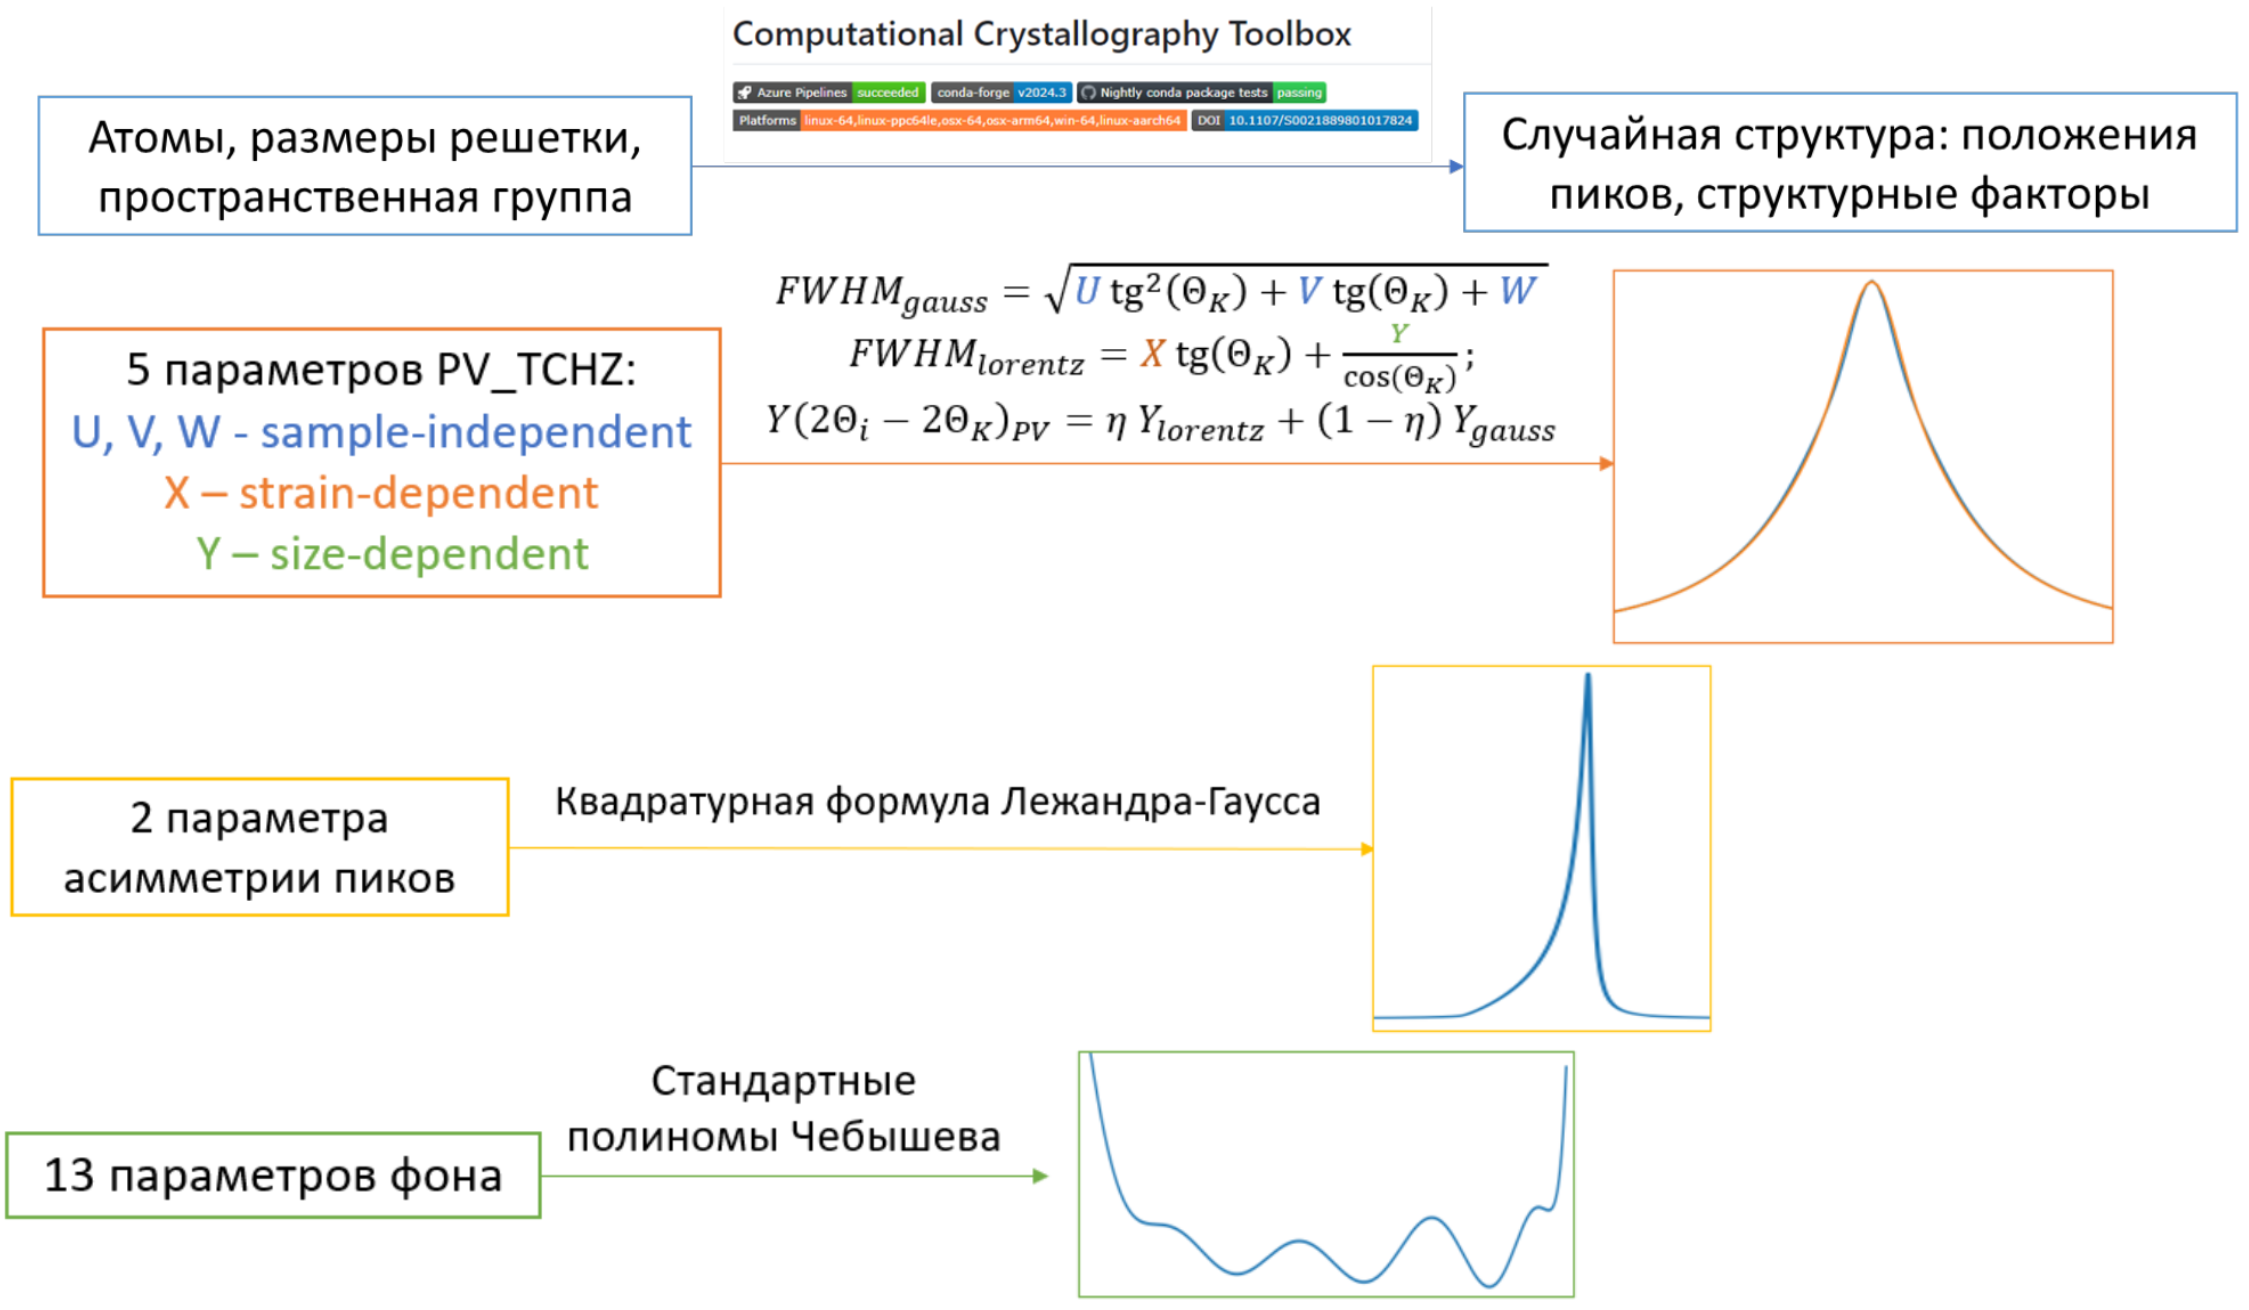
\includegraphics[width=1\textwidth]{figures/pxrd.png}\hfill
	\caption{Схема генерации случайных дифрактограмм в разработанной программе генерации}
	\label{pxrd}
\end{figure}

Начальное обучение моделей глубокого обучения было решено проводить на синтетических структурах, которые были получены с помощью созданного генератора. Так как общее количество симметрично независимых отражений зависит от класса Лауэ, было решено сосредоточиться на моноклинных структурах, поскольку моноклинные группы симметрии являются одними из наиболее распространенных для белковых структур в базе данных белков (\url{rcsb.org/stats/distribution-space-group}). При генерации структур её основные параметры (группа симметрии, типы атомов, их количество) определяются случайным образом (случайное сэмплирование) из следующих значений: 

\begin{itemize}
\item группы симметрии: P2$_1$, C2;
\item атомы: C, N, O, Cl, Br;
\item число симметрично независимых атомов в ячейке: 10--30;
\end{itemize}

600.000 полученных структур были разделены на наборы следующих размеров: 400.000, 100.000 и 100.000 для тренировочной, валидационной и тестовой выборок, соответственно. Были рассчитаны наборы структурных факторов для каждого синтетического образца, разрешение рентгенодифракционных данных было ограничено значением 0.8 \angstrom , карты Паттерсона, а также нормализованные амплитуды структурных факторов.

Также в работе использовались реальные моноклинные молекулярные структуры малых молекул из Кембриджского Банка Структурных Данных \cite{groom_cambridge_2014}, для которых были расчитаны дифракционные отражения. 10.000 структур использовались для дообучения моделей на реальных структурах, 2000~--- были отложены для тестирования.

При выполнении численных экспериментов со структурными факторами было решено работать с их амплитудами. Типичные распределения этих данных для сгенерированных структур представлены на рис. \ref{F_dist}. Как можно заметить, распределение амплитуд более пологое, чем интенсивностей, поэтому именно амплитуды были выбраны для решения задачи. 


\begin{figure}[H]
			\centering
            %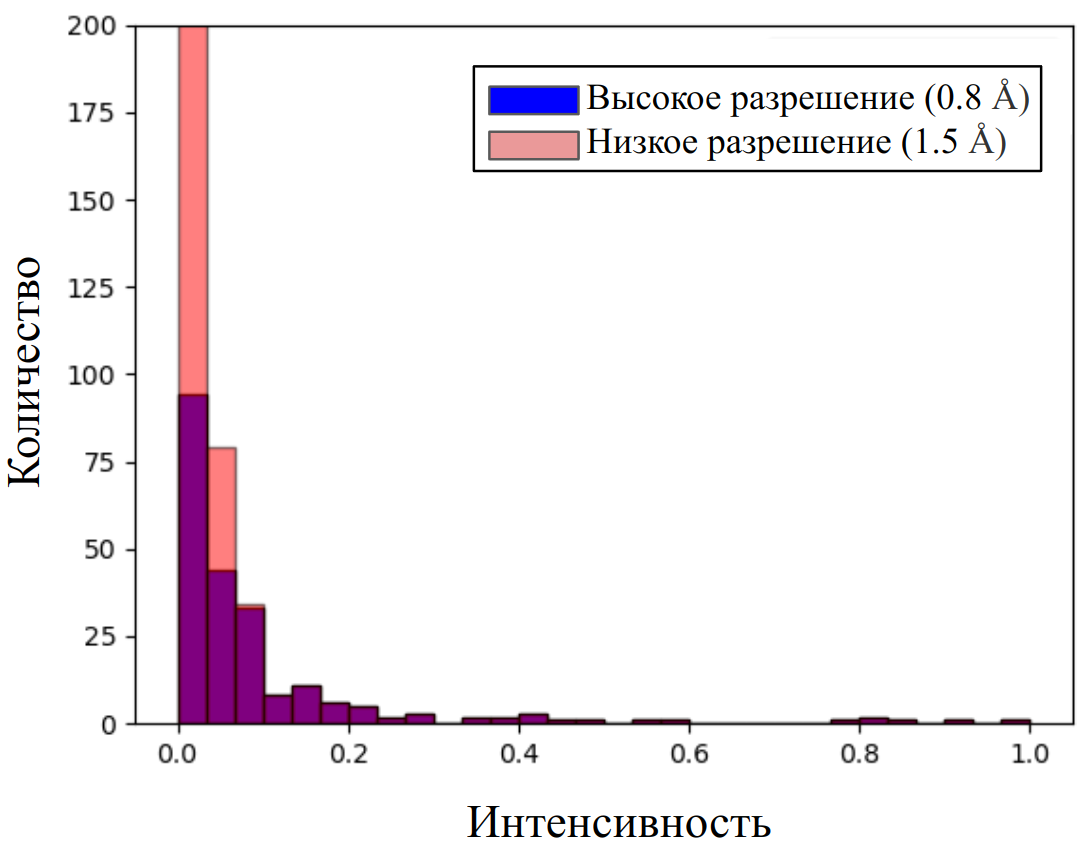
\includegraphics[width=.5\textwidth]{figures/F2_distribution.png}\hfill
            %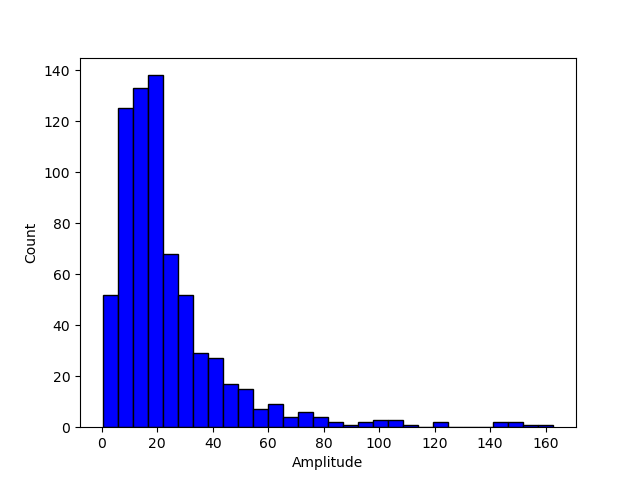
\includegraphics[width=.5\textwidth]{figures/F_distribution.png}
            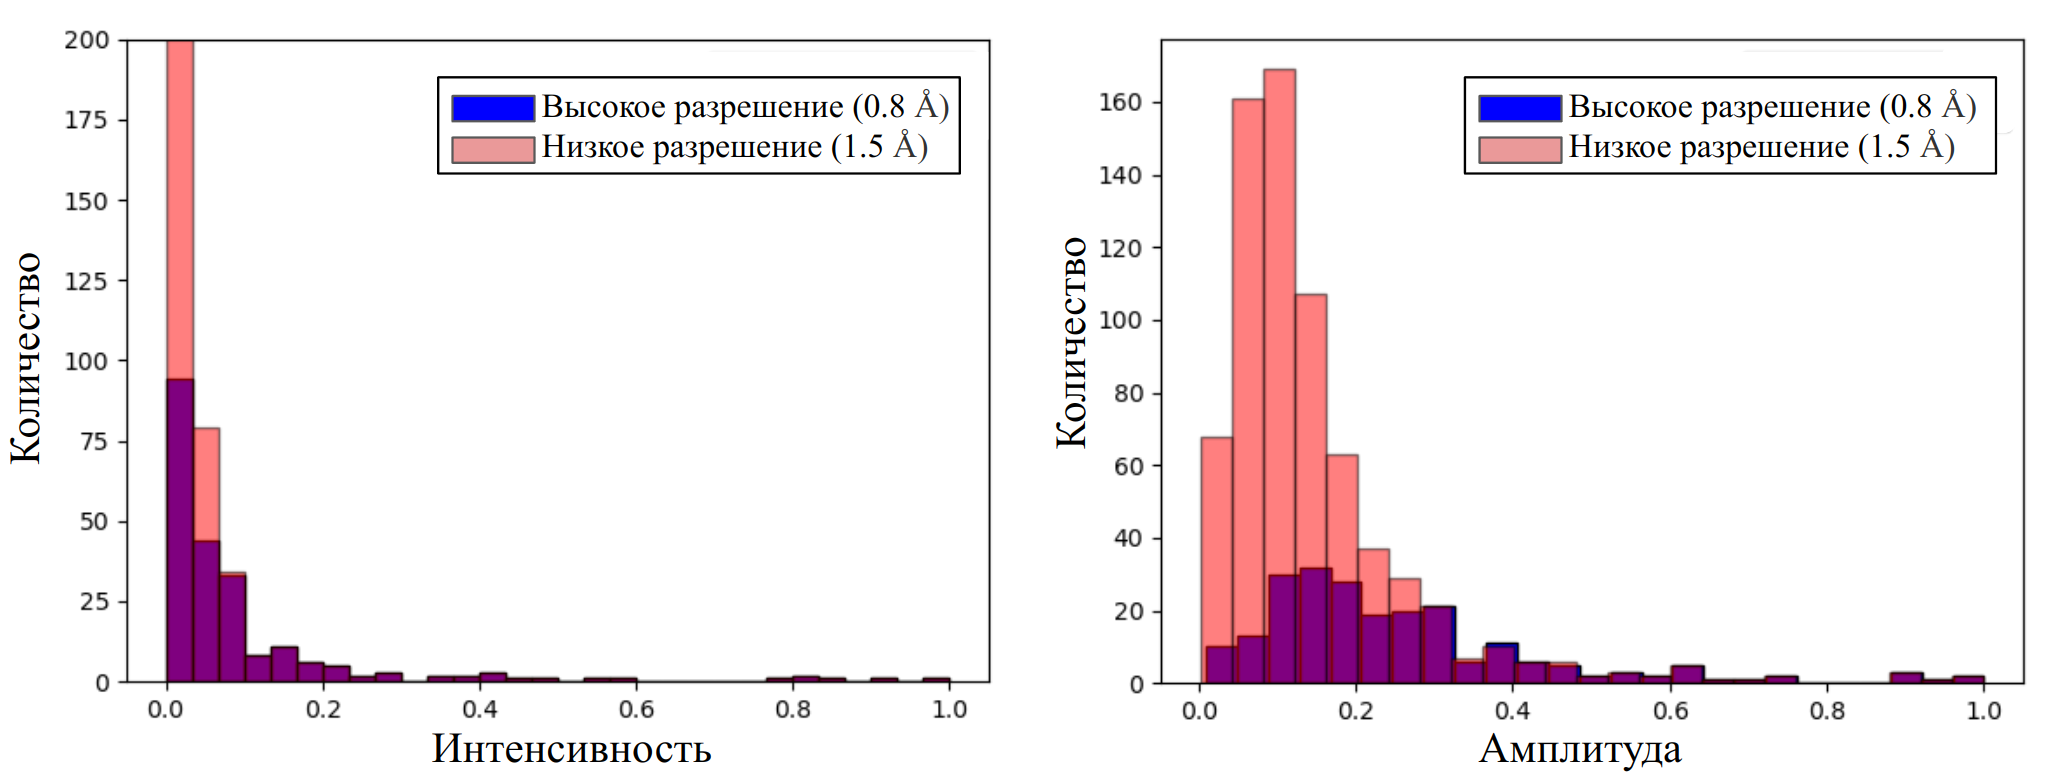
\includegraphics[width=1\textwidth]{figures/F_both.png}
            \caption{Типичные распределения интенсивностей (слева) и амплитуд (справа) дифракционной картины}
            \label{F_dist}
\end{figure}
 

\subsection{Модели}

В качестве базовой модели (baseline) была обучена модель UNet \cite{ronneberger_u-net_2015}, адаптированная для трехмерных данных (рис. \ref{unet}). Данная модель выбрана, потому что она хорошо себя проявляет в простейших задачах увеличения разрешения изображения за счет генерации недостающих пикселей на входных данных низкого разрешения (Super Resolution), однако в данной задаче она не достигает высокой точности восстановления изображения из-за локальной несвязанности рентгенодифракционных данных. 

\begin{figure}[H]
    \centering
    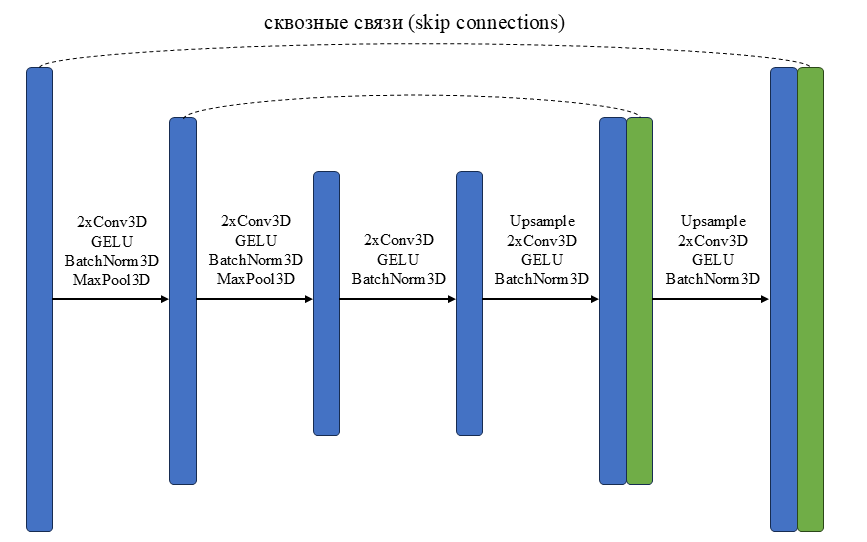
\includegraphics[width=0.8\textwidth]{figures/unet_arch.png}
    \caption{Схемы архитектуры модели UNet}
    \label{unet}
\end{figure}

Также была разработана и обучена модель на основе UNet с улучшенными слоями, содержащими Фурье-преобразование FFT\_UNet (рис. \ref{fft_unet}). Данный подход был продемонстрирован \cite{yang_hionet_2023} при работе с дифракционными данными и он является многообещающим и для нашей задачи, поскольку при переходе в прямое пространство наши данные являются локально связанными.


\begin{figure}[H]
    \centering
    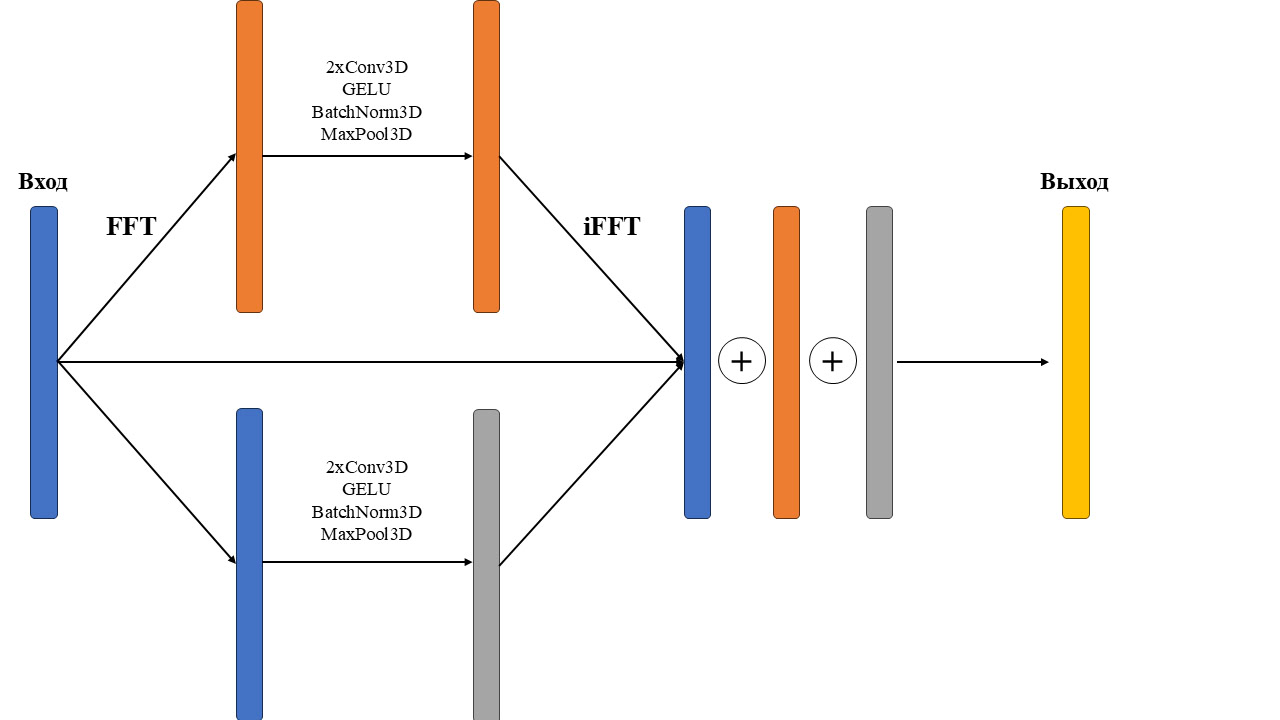
\includegraphics[width=1\textwidth]{figures/fft_arch.jpg}
    \caption{Схема слоёв с преобразованием Фурье}
    \label{fft_unet}
\end{figure}

Поскольку тензоры отражений не являются локально связанными, актуально использование механизма внимания. Он позволит модели находить связи между дальними отражениями. Так, был разработан трансформер XRD\_Transformer для нашей задачи (рис. \ref{XRDTrans}). 

\begin{figure}[H]
    \centering
    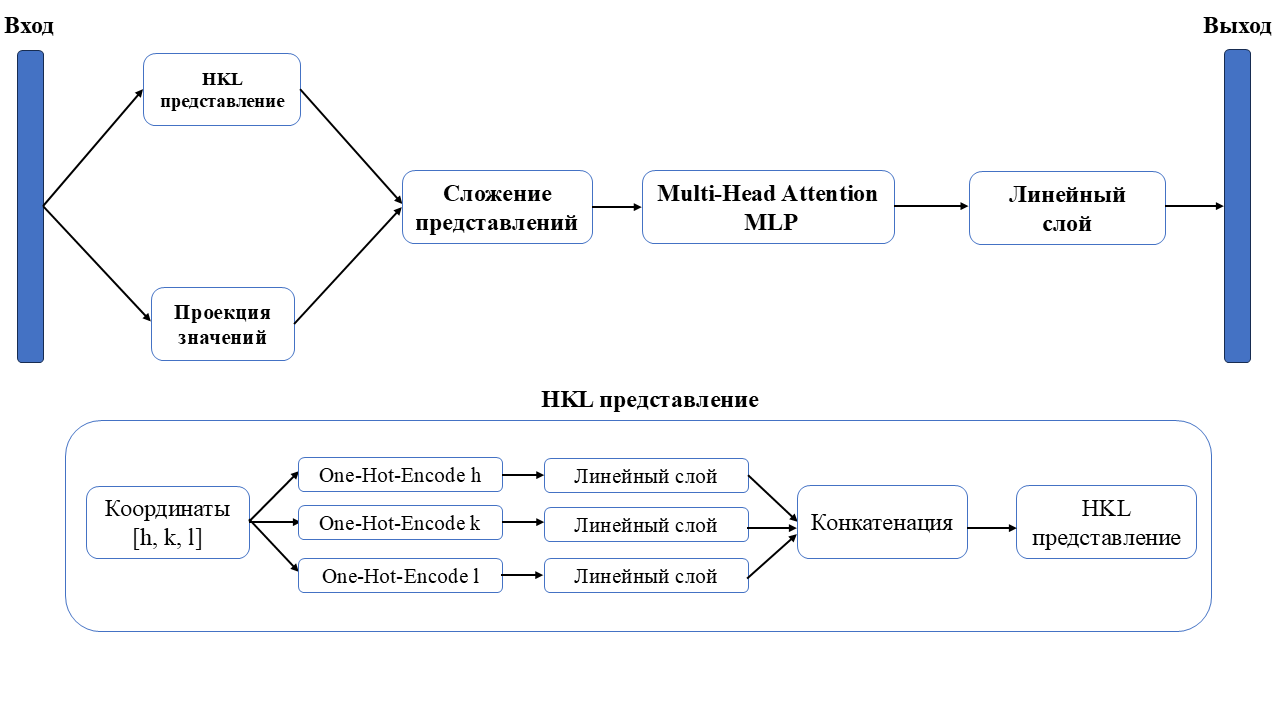
\includegraphics[width=1\textwidth]{figures/xrd_arch.png}
    \caption{Схема архитектуры XRD\_Transformer}
    \label{XRDTrans}
\end{figure}

В модели формируется единое векторное представление (embedding) из индексов Миллера и проекции значений амплитуды отражений, затем он проходит через 5 слоев трансформера, которые состоят из слоев многоголового внимания (Multi-Head Attention) и блоков полносвязных слоев (MLP). Затем после нормализации (LayerNorm) и обратного проецирования в исходное пространство получается восстановленный тензор дифракционной картины.

Так как нам известны все возможные значения индексов Миллера (h, k, l) для структур выбранных размеров с заданным разрешением, HKL представления (рис. \ref{XRDTrans}) формируется следующим образом: индексы кодируются с помощью унитарного кодирования (One-Hot Encoding), после чего каждый вектор с помощью обучаемого линейного слоя проецируется в вектор размерности $\frac{embed_dim}{3}$ после конкатенации размерность полученного векторного представления составляет $embed_dim$. Также в модели реализована возможность получения представления через полносвязный слой, который проецирует позицию (h, k, l) сразу в вектор, однако она не использовалась при обучении модели, так как первый способ является более физическим для нашей задачи, поскольку мы используем только симметрически независимые отражения.


\begin{figure}[H]
    \centering
    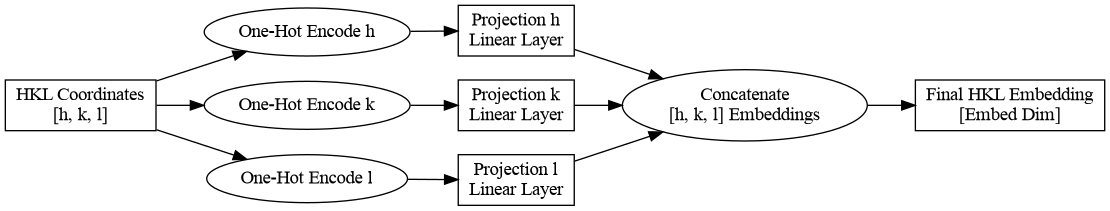
\includegraphics[width=1\textwidth]{figures/hkl_embedding_process.png}
    \caption{Схема формирования эмбеддинга HKL}
    \label{hklembed}
\end{figure}

В качестве функции потерь была выбрана среднеквадратичная ошибка, минимизация которой должна приводить к восстановлению тензора рентгеновских отражений. В качестве метрики для оценки эффективности моделей используется R-фактор: $R = \frac{\sum |F_{obs} - F_{calc}|}{\sum |F_{obs}|}$, где $|F_{obs}|$ --- экспериментальные структурные факторы, $|F_{calc}|$ --- рассчитанные структурные факторы. R-фактор является общепринятым стандартом в кристаллографическом сообществе для оценки качества структурных моделей. Нулевое значение R-фактора отвечает идеальному соответствию между данными модельной структуры и экспериментальными данными.

Также в качестве метрики сравнения изображений рассматривался SSIM \cite{zeng_3d-ssim_2012}, который зарекомендовал себя как хорошая метрика для оценки восстановления и увеличения разрешения изображений, однако эксперименты с ним в качестве добавки к функции потери привели к более низкому качеству восстановления модели с точки зрения R-фактора. Данный результат можно объяснить отсутствием локальной связанности наших данных.
